% vim: set sts=4 et :
\documentclass[aps,prd,reprint,nofootinbib,preprintnumbers]{revtex4}

\usepackage{amsfonts}
\usepackage{amsmath}
\usepackage{graphicx}
\usepackage[svgnames]{xcolor}
\usepackage{hepparticles}
\usepackage{hepnicenames}
\usepackage{hepunits}
\usepackage{graphicx}
\usepackage{caption}
\usepackage{subcaption}
\usepackage{epstopdf}
%% Shortcuts %%
\newcommand{\rmdx}[1]{\mbox{d} #1 \,} % differential
\newcommand{\refapp}[1]{app.~(\ref{app:#1})}
\newcommand{\refeq}[1]{eq.~(\ref{eq:#1})}
\newcommand{\refsec}[1]{sec.~(\ref{sec:#1})}
\newcommand{\reftab}[1]{tab.~(\ref{tab:#1})}
\newcommand{\ie}{\textit{i.e.}}
\newcommand{\nuvec}{\vec{\nu}}
\newcommand{\thvec}{\vec{\vartheta}}
\let\oldtheta\theta
\renewcommand{\theta}{\vartheta}
%\newcommand{\GeV}{\text{GeV}}
\newcommand{\order}[1]{\mathcal{O}\left({#1}\right)}
\let\eps\varepsilon
\newcommand{\aver}[1]{\langle #1 \rangle}
\newcommand{\est}[1]{\widehat{#1}}
\newcommand{\wwhat}[1]{\widehat{\widehat{#1}}}
\DeclareMathOperator{\cov}{Cov}
%\DeclareMathOperator{\skew}{Skew}
\DeclareMathOperator{\kurt}{Kurt}

%% Draft Macros %%
\newcommand{\todo}[1]{{\color{red}\bf ToDo: #1}}
\newcommand{\danny}[1]{{\color{purple}#1}}
\newcommand{\fred}[1]{{\color{brown!85!black}#1}}
\newcommand{\nico}[1]{{\color{green!85!black}#1}}
\newcommand{\citeneeded}{{\color{red}\bf [cite needed]}}

\captionsetup{compatibility=false}

\begin{document}

\allowdisplaybreaks

\preprint{SI-HEP-2014-17}
\title{Extracting Angular Observables without a Likelihood\\and Applications to Rare Decays}
\author{Frederik Beaujean}
\email{frederik.beaujean@lmu.de}
\affiliation{C2PAP, Universe Cluster, Ludwig-Maximilians-Universit\"at M\"unchen, Garching, Germany}
\author{Marcin Chrzaszcz}
\email{mchrzasz@cern.ch}
\author{Nicola Serra}
\email{nicola.serra@cern.ch}
\affiliation{Physik-Institut, Universit\"at Z\"urich, Z\"urich, Switzerland}
\author{Danny van Dyk}
\email{vandyk@tp1.physik.uni-siegen.de}
\affiliation{Theoretische Physik 1, Naturwissenschaftlich-Technische Fakult\"at,
Universit\"at Siegen, Siegen, Germany}

\begin{abstract}
In this letter we study how to obtain a set of angular observables
$\{S_i\}$ that arise in a generic multi-body process without the need
to carry out a likelihood fit of an angular distribution to the
measured events. Instead, we present a method that only relies on
orthogonality of angular functions, and estimation of integrals
by means of Monte Carlo techniques. Beyond providing estimators
for central values and uncertainties, we provide means to determine
the correlation between all angular observables. We show that detector
acceptance effects can be accounted for in the analysis.
\end{abstract}

\maketitle

\section{Introduction}
\label{sec:intro}

The initial motivation for studying what we wish to call the \emph{Method of Moments}
is the determination of angular observables in the rare decay FCNC-mediated decay
$\bar{B}\to \bar{K}^*(\to \bar{K}\pi)\ell^+\ell^-$. However, we emphasize that
the method we describe in this letter is general, and it applies to arbitrary
decay or scattering processes. We find a previous work \cite{Dighe:1998vk}
advocates this method chiefly for the determination of angular observables in non-leptonic
$B$ decays, but also mentions the applicability to semileptonic decays. We improve
upon this previous work by studying correlations between the angular observables,
and sources of systematic uncertainties. Moreover, we will show that the method
at hand has two benefits over the usual approach based on likelihood fits.
\begin{enumerate}
    \item Likelihood fits do not always converge. \fred{Why? Mismodelling? Expand!}
    \item Using the method at hand, the joint probability distribution of the
        angular observables converges towards a multivariate normal distribution.
        This allows easy transfer of information from the experiment to interest
        theorists.
\end{enumerate}


We continue with basic definitions that pertain to angular observables, and our
results in the subsequent sections. Let $\thvec = (\theta_1, \dots \theta_N)$ denote the set of all
angles, and let $\nuvec = (\nu_1, \dots \nu_M)$ denote the set of all
other non-angular kinematic variables needed to fully specify the
final state of the process under study. For example, $\nuvec$ may
include invariant masses or center-of-mass energies. We define an
angular observable $S_i$ as a coefficient in the probability density
function (PDF) of the process by means of
\begin{align}
    \label{eq:def-P}
    P(\nuvec, \thvec) \equiv \sum_i S_i(\nuvec) \times f_i(\thvec)\,.
\end{align}
Here, the dependence on the $n$ decay angles $\thvec$ has been
explicitly factored out in terms of the angular functions
$f_i(\thvec)$, which we assume to fulfill the orthonormality relations
\begin{equation}
    \label{eq:def-ortho-rel}
    \int_\Omega \rmdx{^N \theta} f_i(\thvec) f_j(\thvec)  = \delta_{ij}\,,
\end{equation}
with $\Omega$ representing the full angular phase space relevant to the process.
For the purpose of this letter, however, it suffices that the system
of angular functions $f_i(\thvec)$ can be transformed into an
orthonormal basis. The transformation needs to be worked out on a
case-by-case basis. For a selection of $B$ decays which we consider the most interesting
we list the transformations in a series of appendices \ref{app:btokll} through
\ref{app:lambdabtolambdall}.\\


For particle decays, $P$ is generally expressed in terms of the fully differential decay width,
\begin{align}
    \label{eq:def-P-decay}
    P(\nuvec, \thvec) \equiv \frac{1}{\Gamma}\frac{\rmdx{^{N+M}\Gamma}}{\rmdx{\nu_1} \dots \rmdx{\nu_M} \rmdx{\theta_1} \dots \rmdx{\theta_N}}\,,
\end{align}
where $\Gamma$ is the total decay width. For a scattering process, one can similarly use
\begin{align}
    \label{eq:def-P-scattering}
    P(\nuvec, \thvec) \equiv \frac{1}{\sigma}\frac{\rmdx{^{N+M}\sigma}}{\rmdx{\nu_1} \dots \rmdx{\nu_M} \rmdx{\theta_1} \dots \rmdx{\theta_N}}\,,
\end{align}
where the total cross section $\sigma$ is used for the
normalization. Since the determination of the total decay width or
total cross section can be quite difficult, we emphasize that
different normalizations for $P$ can be used.  For instance, the total
decay width (or cross section) of the process of interest can be
replaced by the corresponding quantity of a control-channel
process. This change of normalization is equivalent to a linear rescaling of
the angular observables $\lbrace S_i\rbrace$; thus ratios or similar suitable combinations
of the angular observables are invariant.\\


In the remainder of this letter we discuss how to obtain the angular
observables $S_i(\nuvec)$ in an experimental setup where each recorded
event is (approximately) distributed according to $P$.  We establish
the statistical basics in section \ref{sec:sample-based-det}. Section
\ref{sec:systematics} is dedicated to the impact of systematic effects
such as mismodeling the underlying physics or detector acceptance
effects. Numerical studies for one uni-angular and one triple-angular
distribution are provided in section \ref{sec:numerics}. In a series
of appendices we provide the orthonormal bases of angular functions
relevant to several rare $b$ decays.



\section{Sample-Based Determination}
\label{sec:sample-based-det}

The orthonormality relations \refeq{def-ortho-rel} imply that a single angular observable $S_i$
can be projected out of the full PDF $P$ by means of
\begin{equation}
    \label{eq:det-Pi-analytical}
    S_i(\nuvec) = \int_{\Omega} \rmdx{^N \theta} \hat{f}_i(\thvec) P(\nuvec, \thvec)\,.
\end{equation}
where $\lbrace \hat{f}_i \rbrace$ denotes a \emph{dual basis} of angular function. In all generality
the bases $\lbrace f_i \rbrace$ and $\lbrace \hat{f}_i \rbrace$ are not identical. This is the
case for our selection of applications in appendices \ref{app:btokll} through \ref{app:lambdabtolambdall}.\\

It is sensible to refer to the angular observable $S_i$ as the \emph{$\hat{f}_i$-moment} of the PDF $P$.
We emphasize that a relation of type \refeq{det-Pi-analytical} holds for any combination of
scalar product and orthonormal basis of angular functions $\lbrace f_i \rbrace$; \ie, there is no unique
basis of angular functions. For the proof we refer to ref. \cite{Dighe:1998vk}.\\
In addition, integration over the non-angular variables yields
\begin{equation}
    \langle S_i\rangle
    \equiv \int \rmdx{^M \nu} S_i(\nuvec)
    = \int \rmdx{^M \nu} \left[\int_{\Omega} \rmdx{^N \theta}\hat{f}_i(\thvec) P(\nuvec,\thvec) \right].
\end{equation}
The remainder of this section describes the method of moments, in which we replace the
analytical integration \refeq{det-Pi-analytical} by Monte Carlo (MC) estimators.\\


The central tenet of MC integration is the fact that the expectation value $E_P[g]$ of some function
$g(x)$ under the probability density $P(x)$,
\begin{equation}
    E_P[g] \equiv \int \rmdx{x} g(x) P(x)
\end{equation}
can be approximated \cite{MCSM-2004} by an MC estimator $\est{E_P[g]}$
\begin{equation}
    \label{eq:mc-id}
    E_P[g] \to \widehat{E_P[g]} \equiv \frac{1}{K} \sum_{k=1} g(x^{(k)})
\end{equation}
due to the strong law of large numbers for $K \to \infty$ assuming
that the variates $x^{(k)}$, $k = 1, \dots, K$ are distributed as
$P$; i.e.,
\begin{equation}
    x^{(k)} \sim P\,.
\end{equation}
Throughout this letter we denote all MC estimators with a wide hat.\\


Application of \refeq{mc-id} then yields
\begin{equation}
    \langle S_i\rangle \to \widehat{\langle S_i\rangle} = \frac{1}{K} \sum_{k=1}^{K} \hat{f}_i(x^{(k)})\,.
\end{equation}
It is often of interest to obtain the $\nuvec$- observables integrated
over certain ranges of $\nuvec$; i.e., binned measurements of $\langle
S_i\rangle$.
Therefore, we introduce the bin-integrated quantity
\begin{align}
    \langle S_i\rangle_{\vec{a},\vec{b}}
    & = \int_{\vec{a}}^{\vec{b}} \rmdx{^M \nu} S_i(\nuvec)\\
    & = \int_{\vec{a}}^{\vec{b}} \rmdx{^M \nu} \left[\int_{\Omega} \rmdx{^N\theta} \hat{f}_i(\thvec) P(\nuvec,\thvec)  \right]\\
    & = \int \rmdx{^M \nu} \left[\int_{\Omega} \rmdx{^N\theta} \hat{f}_i(\thvec) P(\nuvec,\thvec)
        \mathbf{1}(\vec{a} \le \nuvec \le \vec{b})\,
        \right],
\end{align}
where the argument of the indicator function $ \mathbf{1}(\vec{a} \le
\nuvec \le \vec{b})$ is to be interpreted componentwise.
Application of \refeq{mc-id} immediately yields
\begin{equation}
    \label{eq:bin-importance}
    \widehat{\langle S_i\rangle_{\vec{a},\vec{b}}}
    = \frac{1}{K} \sum_{k=1}^{K} \hat{f}_i(x^{(k)})         \mathbf{1}(\vec{a} \le \nuvec \le \vec{b})\,.
\end{equation}
This basically reduces the estimation of
$\aver{S_i}_{\vec{a},\vec{b}}$ to a (weighted) counting experiment. In
the limit $N \to \infty$, the random vector $( \dots,
\aver{S_i}_{\vec{a},\vec{b}}, \dots)$ follows a multivariate Gaussian
distribution \citeneeded\fred{Robert,Casella?}
with the mean vector estimated by \refeq{bin-importance}, and the covariance
estimated as
\begin{equation}
    \cov[\aver{S_i},\aver{S_j}]_{\vec{a},\vec{b}} \to \est{\cov}[\aver{S}_i, \aver{S}_j]_{\vec{a},\vec{b}}
        = \frac{1}{K - 1} \sum_{k=1}^{K} \big[\hat{f}_i(x^{(k)}) - \est{\langle S_i\rangle_{\vec{a},\vec{b}}}\big]\,\big[\hat{f}_j(x^{(k)}) - \widehat{\langle S_j\rangle_{\vec{a},\vec{b}}}\big]
        \mathbf{1}(\vec{a} \le \nuvec \le \vec{b})\,.
\end{equation}
We would like to emphasize that the sample covariance should rapidly converge towards the true covariance matrix.
We propose to declare convergence once estimators for skewness and kurtosis are sufficiently small,
\begin{equation}
    \est{\operatorname{Skew}}[\aver{S_i},\aver{S_j}] \ll 1\,\,\text{ and }\,\,\est{\kurt}[\aver{S_i},\aver{S_j}] \ll 1\,.
\end{equation}

The convergence towards a normal distribution for the results allows to transfer correlation information to interested
theorists. In particular, this will allow to constrict predictive distributions of optimized observables.
(See e.g. \cite{Egede:2008uy,Egede:2010zc,Bobeth:2010wg,Becirevic:2011bp,Bobeth:2012vn,Matias:2012xw,DescotesGenon:2012zf}
for definitions of such optimized observables in $B\to K^*\ell^+\ell^-$ decays, \cite{Faller:2013dwa} for application to
the decay $B\to \pi\pi\ell^-\bar\nu_\ell$, and \cite{Boeer:2014xx} for observables in $\Lambda_b\to\Lambda(\to N\pi)\ell^+\ell^-$).



\section{Sources of Systematic Uncertainties}
\label{sec:systematics}

In \refsec{sample-based-det}, we assume that the PDF $P$ describe the underlying physics accurately,
and that the experiment observes each event with perfect accuracy. In order to estimate systematic
uncertainties, we lift these assumptions.

\subsection{Mismodeling due to Contributions by Higher Partial Waves}
\label{sec:systematics:partial-waves}

\begin{figure}
    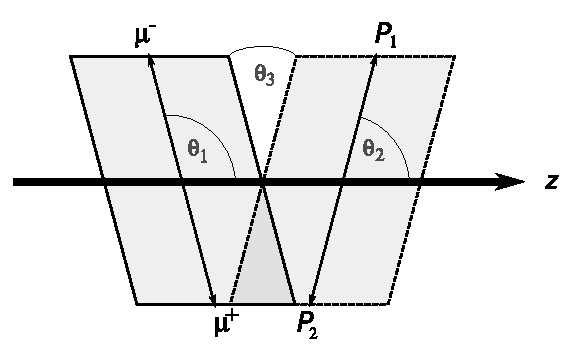
\includegraphics[width=.6\textwidth]{fig-topology.pdf}
    \caption{Decay topology for decays $B\to P_1 P_2 \ell_1 \bar\ell_2$. \label{fig:topology}}
\end{figure}

So far, we assumed that our underlying physical process was accurately described by our PDF $P$.
However, in several interesting processes we might only have an approximative result for $P$.
In this section, we take the interesting class of four-body decays $B\to P_1 P_2 \ell_1 \bar\ell_2$
as an example\footnote{This includes the rare $b\to s$ mediated $B$ decay $B \to K\pi\ell^+\ell^-$, and
the $V_{ub}$ suppressed decay $B\to \pi\pi\ell^+\bar\nu_\ell$. For both examples the PDF $P$ is known in
the small-width approximation and when assuming a pure $P$-wave, resonant final state. An extension to
$S-P$ interference has been studied for $B\to K\pi\ell^+\ell^-$ \cite{Blake:2012mb,Becirevic:2011bp},
and for $\bar{B}\to \pi\pi\ell^-\bar\nu_\ell$ \cite{Faller:2013dwa}. For a first study of $S$, $P$
and $D$ interference, see \cite{Das:2014sra}}.%
The PDFs for these decays are usually expressed in terms of one or a few partial waves
of the dimeson system. However, the angular momentum of the dimeson system is unbounded from above.
\\

For the selected class of decays, we face the problem that $P$ has a given dependence on the dilepton
helicity angle $\theta_1$ and the azimuthal angle $\theta_3$. (See also \refapp{btokpill} for details
on the angular distribution.) However, on the level of decay amplitudes the dimeson system can have an arbitrary
large total angular momentum $j$; only its third component is restricted to $m = -1,0,+1$.\\

We advocate here that is a sensible procedure to perform an expansion in terms of Legendre polynomials $p_{j}^{(|m|)}$
with respect to the remaining angle $\theta_2$. Using the observables $S_k(\vec{\nu})$, $k=1,\dots,9$, with $\vec{\nu}=(q^2, k^2)$
and as defined in \refapp{partial-waves}, the expansion reads
\begin{equation}
    S_{k}(\vec{\nu},\cos\theta_2) \equiv \sum_{j} \frac{1}{n_{j,|m|}} S_{k,j}(\vec{\nu}) p_{j}^{(|m|)}(\cos\theta_2)\sin\theta_2\,,
\end{equation}
where the the normalization factor $n_{j,|m|}$ is defined in \refeq{legendre-scalar-product}, and we have
\begin{equation}
    |m| = \begin{cases}
        0\,, & k = 1,2,6\,\\
        1\,, & k = 3,4,5,7,8,9\,,
    \end{cases}\,.
\end{equation}
The angular observables $S_{k,j}$ defined as coefficients of this expansion
have the merit of a well-defined total angular momentum, and thus are physically discriminable.
As a consequence of the orthogonality of the Legendre polynomials, any mismodelling (or rather, lack of modelling of higher
partial-wave observables) \emph{does not affect} the method of moments as discussed in the previous section.\\

Unfortunately, this benefit on the experimental side is accompanied with a theoretical draw back. Each observable
$S_{k,j}(\vec{\nu})$ consists of an infinite sum of bilinear of partial-wave amplitudes. It remains for theoretical
analyses to estimate or calculate the impact of partial waves beyond the S and P wave contributions.
(For $B\to K\pi\ell^+\ell^-$ a first study has been carried out where contributions up to the D wave are studied \cite{Das:2014sra}).\\

We wish to emphasize, however, that detector acceptance effects systematically affect the expansion for any basis
of angular functions. The means to cope with this problem are discussed in the following subsection.


\subsection{Detector Acceptance Effects}
\label{sec:systematics:acceptance}

\paragraph{Recipe to determine the acceptance effects}

The determination of detector acceptance is generally a difficult
task. Here, we will show a systematic method to estimate its effects
based on both the method of moments, and MC simulations of the
detector.

\fred{In the ideal case, one would have an explicit probabilistic
  model of the detector acceptance effects and could thus write down
  the full forward model of the measured events arise. In practice,
  this would require much more CPU time than available, and one is
  therefore forced to simplify the model. The standard approach is to
  generate \emph{true} particle events $\lbrace x_t^{(k)}\rbrace =
  \lbrace(\vec{\nu}^{(k)}_t,\vec\theta^{(k)}_t)\rbrace$ from a PDF
  assumed to describe the bare physical process, and to propagate
  those particles through a detailed simulation of the detector. The
  observable traces that the particles leave in the detector are fed
  into reconstruction algorithms resulting in the \emph{detector}
  events $\lbrace x^{(k)}_d\rbrace = \lbrace(\vec{\nu}^{(k)}_d,
  \vec\theta^{(k)}_d)\rbrace$.

[Where does the reconstruction uncertainty enter? Below we just
  account for systematic shifts but our estimate of the uncertainty of
  one $S_k$ would be only the statistical uncertainty from the finite
  sample size. How about the extra correlation between different $S_k$
  that is induced?] }\\

As before, we assume a PDF $P$ can be decomposed into $N$ parts with angular observables $\lbrace S_k\rbrace$,
\begin{equation}
    P \equiv P(\vec\nu,\vec\theta | \lbrace S_k \rbrace)\,.
\end{equation}
We denote the estimator of an
observable $S_k$ as $\est{S_k}$, which is affected by the detector acceptance. We assume now that there is a linear relation
between the true angular observables $\lbrace S_k^\text{true}\rbrace$, and the estimators $\lbrace \est{S_k}\rbrace$,
\begin{equation}
    \label{eq:linear-assumption}
    \est{S_i} = \sum_{i = 1}^N M_{i j} S_j^\text{true}\,.
\end{equation}
This assumption is based on a smooth angular acceptance function. While this will not be true for the laboratory frame,
smoothness may be recovered in boosted frame, e.g. the rest frame of the decaying particle.
In that case, the matrix $M_{ij}$ can be fully determined through the following steps.
\begin{enumerate}
    \item For a fixed $j$, let $S_j^\text{true} = 1$, and $S_k^\text{true} = 0\,\forall k\neq j$.
    \item Draw simulated events $\lbrace x_t^{(k)}\rbrace = \lbrace(\vec{\nu}^{(k)}_t,\vec\theta^{(k)}_t)\rbrace$ (dubbed ``true'') from the PDF $P_j$,
        \begin{equation}
            P_j \equiv P(\vec\nu,\vec\theta | \lbrace S_j = 1, S_{k\neq j} = 0\rbrace)\,.
        \end{equation}
    \item Use the true events as input for the MC simulation of the detector, in order to obtain the detector
        events $\lbrace x^{(k)}_d\rbrace = \lbrace(\vec{\nu}^{(k)}_d,\vec\theta^{(k)}_d)\rbrace$.
    \item Use the method of moments to determine the uncorrected observables $\lbrace \est{S_k} \rbrace$, based on the detector
        events $\lbrace x^{(k)}_d\rbrace$.
    \item By virtue of \refeq{linear-assumption} and step 1, the $j$-th column of $M$ has been determined via
        \begin{equation}
            M_{ij} = \est{S_i}\,.
        \end{equation}
        \fred{I wonder if a small sample size also leads to artificial
          nonzero off-diagonal elements of $M$}
    \item Repeat the above steps for all values of $j$ to determine all columns of $M$.
\end{enumerate}

It remains to invert the relation \refeq{linear-assumption}, so that one can determine the unfolded
angular observables $\lbrace \wwhat{S_k}\rbrace$ as
\begin{equation}
    \wwhat{S_i} = \left(M^{-1}\right)_{ij} \est{S_j}\,.
\end{equation}

We emphasize that this methods hinges on the assumption in \refeq{linear-assumption}, We thus suggest to explicitly
test the assumption. One way of testing involves repeating the previous procedure
with $S_j^\text{true} = 1/x$. If the lineary assumption holds, one should find
\begin{equation}
    M_{ij} = x \est{S_i}\,,
\end{equation}
for arbitrary values of $x > 1$.


\section{Toy Studies}
\label{sec:numerics}

In order to study the performance of the proposed method, we simulate measurements for one uni-angular
and one tri-angular decay distribution for various numbers of events. As inputs we use the SM predictions
for the decays $B\to K\ell^+\ell^-$ and $B\to K^*(\to K\pi)\ell^+\ell^-$, respectively. We cover the
$q^2$ ranges $1\GeV^2$ to $6\GeV^2$, and $15\GeV^2$ to to the respective kinematic endpoint, with two
bin widths: $1\GeV^2$ and $0.5\GeV^2$. This is to ensure that a wide spectrum of possible values for
the angular observables. We find:
\begin{itemize}
    \item In all studied cases we observed not a single bias in the pull distribution of the observable.
    \item The error $\sigma_k(N)$ of an angular observable $S_k$, evaluate for $N$ events is very well
        fitted by
        \begin{equation}
            \sigma_k(N) = \frac{\sigma_k(1)}{\sqrt{N}}
        \end{equation}
        with $\sigma_k(1) = \order{1}$. \todo{Check this!}
    \item \todo{Plot Skewness and Kurtosis for $S_5$ and $S_7$ as functions of $N$.}
    \item \todo{Perform Mardia's Skewness and Kurtosis tests.}
    \item \dots
\end{itemize}
We find that all of the above results show consistenly convergence of the distribution for the angular observables
towards a multivariate normal distribution.

\begin{figure}[t]
        \centering
        \begin{subfigure}[b]{0.45\textwidth}
                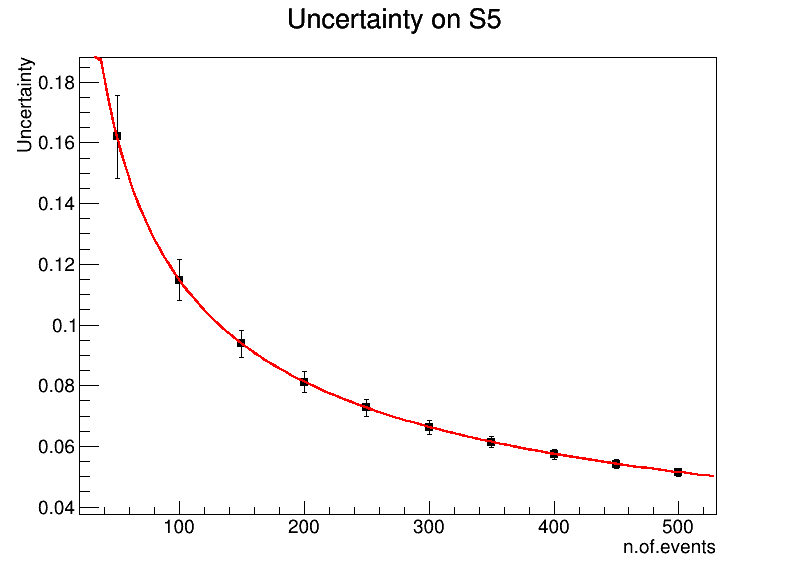
\includegraphics[width=0.8\textwidth]{figs/Q2_5_6_S5.png}
        \end{subfigure}
        \begin{subfigure}[b]{0.45\textwidth}
                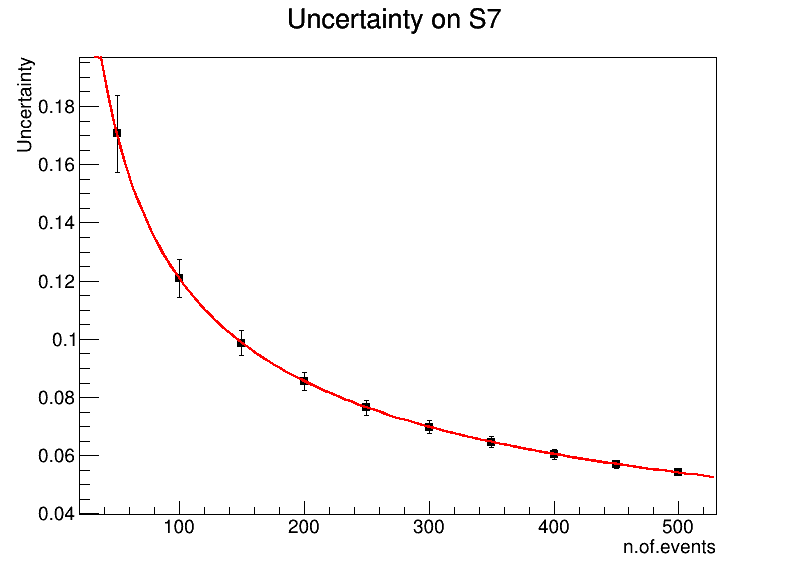
\includegraphics[width=0.8\textwidth]{figs/Q2_5_6_S7.png}
        \end{subfigure}
        \caption{Uncertainty of the angular observables $S_5$ and $S_7$, extracted from simulated events of the decay $B\to K^*\ell^+\ell^-$
        and as a function of the number of simulated events $N$. The red curve represents a fit to the function $\sigma_k(N) = \frac{\sigma_k(1)}{\sqrt{N}}$.}
        \label{fig:errors}
\end{figure}


We used the simulated events and fitted a likelihood function to them.
\begin{itemize}
    \item For a small number of simulated events, \danny{$N=?$}, we observe a significant bias in the pull distributions.
    \item For a large number of simulated events, \danny{$N=?$}, the uncertainty of the angular observables is
        smaller compared to the results of the method of moments.
\end{itemize}
\todo{compare robustness to likelihood fit when fit doesn't
converge. Why exactly doesn't it converge? What if physics model
wrong, say some angular terms are missing.}


\section{Conclusion}

In this letter \dots
\begin{enumerate}
    \item errors on the means are in very good approximation gaussian.
    \item correlation are small and faithfully model a multivariate gaussian. \fred{$\Rightarrow$ easy transfer of knowledge to theory fits}
\end{enumerate}


\acknowledgments

The work of D.v.D has been supported by the Bundesministerium f\"ur Bildung und Forschung (BMBF).
\dots
\danny{Potential people to read the manuscript: Jochen Dingfelder (Belle-II, Bonn), Ulrik Egede (LHCb, Imperial London), Christoph Langenbruch (LHCb, Warwick), Michel De Cian (LHCb, Heidelberg), Adrian Bevan (ATLAS, Queen Mary)  }
D.v.D would like to thank Gudrun Hiller and Martin Jung for discussing the results of \cite{Das:2014sra} prior to publication.

\appendix

\section{Application to $\bar{B}\to\bar{K}\ell^+\ell^-$}
\label{app:btokll}

The PDF for the decay $\bar{B}\to\bar{K}\ell^+\ell^-$ has been calculated for the most
complete basis of dimension-six $b\to s \ell^+\ell^-$ operators. It reads \cite{Bobeth:2007dw,Bobeth:2012vn}
\begin{equation}
    P(q^2, \cos\theta_1) = \frac{1}{\Gamma} \frac{\rmdx{^4\Gamma}}{\rmdx{q^2} \rmdx{\cos\theta_1}} = \frac{a(q^2)}{\Gamma} + \frac{b(q^2)}{\Gamma} \cos\theta_1 + \frac{c(q^2)}{\Gamma} \cos^2\theta_1 = \sum_i P_i f_i(\cos\theta_1)\,,
\end{equation}
where the basis of angular functions $\lbrace f_i\rbrace$ reads
\begin{equation}
\begin{aligned}
    f_1 & = 1\,, &
    f_2 & = \cos\theta_1\,, &
    f_2 & = \cos^2\theta_1\,.
\end{aligned}
\end{equation}
Here we denote the dilepton mass squared as $q^2$, and the dilepton helicity angle as $\theta_1 \equiv \theta_{\ell}$. We transform the PDF from a $\cos\theta_1$-dependence
to a $\theta_1$-dependence,
\begin{equation}
    P(q^2, \theta_1) = \sum_i P_i f_i(\cos\theta_1) \sin \theta_1\,.
\end{equation}
where we define $P_{\lbrace 1,2,3\rbrace} \equiv \lbrace a, b, c\rbrace / \Gamma$.\\

The dual basis $\lbrace \hat{f}_i\rbrace$ reads
\begin{equation}
\begin{aligned}
    \hat{f}_1 & = \frac{9}{8} - \frac{15}{8}\cos^2\theta_1\,, &
    \hat{f}_2 & = \frac{3}{2}\cos\theta_1\,, &
    \hat{f}_3 & = -\frac{15}{8} + \frac{45}{8}\cos^2\theta_1\,,
\end{aligned}
\end{equation}
such that
\begin{equation}
    \int_0^\pi \rmdx{\theta_1} \hat{f}_i(\theta_1) P(q^2, \theta_1) = S_i(q^2)\,.
\end{equation}

\section{Application to $\bar{B}\to\bar{K}\pi\ell^+\ell^-$ (S-wave and P-wave)}
\label{app:btokstarll}

The PDF for the decay $\bar{B}\to\bar{K}\pi\ell^+\ell^-$ --- up to and including P-wave contributions --- has been calculated
for the most general basis of dimension-six $b\to s$ operators. It reads, expressed in terms of the angular observables $\lbrace J_i\rbrace$ \cite{Blake:2012mb,Bobeth:2012vn}
\begin{equation}
    P(q^2, \cos\theta_1, \cos\theta_2, \theta_3) = \frac{1}{\rmdx{\Gamma}/\rmdx{q^2}} \frac{\rmdx{^4\Gamma}}{\rmdx{q^2} \rmdx{\cos\theta_1} \rmdx{\cos\theta_2} \rmdx{\theta_3}} = \frac{3}{8\pi} \sum_k \frac{J_{k}(q^2)}{\rmdx{\Gamma} /\, \rmdx{q^2}} f_k(\cos\theta_1, \cos\theta_2, \theta_3)\,,
\end{equation}
where $\theta_1 \equiv \theta_\ell$ is the dilepton helicity angle, and $\theta_2 \equiv \theta_{K}$ is the $\bar{K}\pi$ helicity angle, and $\theta_3 \equiv \phi$ is the azimuthal angle.
The $q^2$-differential decay width reads
\begin{equation}
    \frac{\rmdx{\Gamma}}{\rmdx{q^2}} = \frac{\big(3 J_{1c} - J_{2c}\big) + 2\big(3J_{1s} - J_{2s}\big)}{3}\,.
\end{equation}
The angular functions\footnote{%
    We consistently use the label "$i$" to denote angular function and observables that arise
    from interference between S-wave and P-wave amplitudes. Our convention is related to the convention
    of \cite{Bobeth:2012vn} through $f_{1i} \leftrightarrow f_{1sc}$, $f_{2i} \leftrightarrow f_{2sc}$.
} read \cite{Blake:2012mb,Bobeth:2012vn}
\begin{equation}
\begin{aligned}
    f_{1s} & = \sin^2\theta_2 &
    f_{1c} & = \cos^2\theta_2 &
    f_{1i} & = \cos\theta_2\\
    f_{2s} & = \sin^2\theta_2 \cos 2\theta_1 &
    f_{2c} & = \cos^2\theta_2 \cos 2\theta_1 &
    f_{2i} & = \cos\theta_2 \cos 2\theta_1\\
    f_{3}  & = \sin^2\theta_2\sin^2\theta_1 \cos 2\theta_3 &
    f_{4}  & = \sin 2\theta_2 \sin 2\theta_1 \cos\theta_3 &
    f_{4i} & = \sin\theta_2 \sin 2\theta_1 \cos\theta_3\\
    f_{5}  & = \sin 2\theta_2 \sin \theta_1 \cos\theta_3 & & &
    f_{5i} & = \sin\theta_2 \sin \theta_1 \cos\theta_3\\
    f_{6s} & = \sin^2\theta_2 \cos\theta_1 &
    f_{6c} & = \cos^2\theta_2 \cos\theta_1\\
    f_{7}  & = \sin 2\theta_2 \sin \theta_1 \sin\theta_3 & & &
    f_{7i} & = \sin\theta_2 \sin \theta_1 \sin\theta_3\\
    f_{8}  & = \sin 2\theta_2 \sin 2\theta_1 \sin\theta_3 & & &
    f_{8i} & = \sin\theta_2 \sin 2\theta_1 \sin\theta_3\\
    f_{9}  & = \sin^2\theta_2\sin^2\theta_1 \sin 2\theta_3\\
\end{aligned}
\end{equation}
We indicate contributions from the interference of S waves and P waves by an index \emph{i}. In terms of the angles $\theta_1$ and $\theta_2$, instead of their cosines, the PDF reads
\begin{equation}
    P(q^2, \theta_1, \theta_2, \theta_3) = \frac{3}{8\pi} \sum_k S_k(q^2) f_k(\cos\theta_1, \cos\theta_2, \phi) \sin\theta_1 \sin\theta_2\,,
\end{equation}
where we also define $S_k(q^2) \equiv J_k(q^2) / (\rmdx{\Gamma} /\, \rmdx{q^2})$.\\

The dual basis reads
\begin{equation}
\begin{aligned}
    \hat{f}_{1s} & = \frac{\big( 63 \sin^2\theta_2 - 42 \cos^2\theta_2\big) + \big(  45 \sin^2\theta_2 - 30 \cos^2\theta_2\big)\cos 2\theta_1}{64} \,,\\
    \hat{f}_{1c} & = \frac{\big(-21 \sin^2\theta_2 + 84 \cos^2\theta_2\big) + \big( -15 \sin^2\theta_2 + 60 \cos^2\theta_2\big)\cos 2\theta_1}{32} \,,\\
    \hat{f}_{2s} & = \frac{\big( 45 \sin^2\theta_2 - 30 \cos^2\theta_2\big) + \big(+135 \sin^2\theta_2 - 90 \cos^2\theta_2\big)\cos 2\theta_1}{64} \,,\\
    \hat{f}_{2c} & = \frac{\big(-15 \sin^2\theta_2 + 60 \cos^2\theta_2\big) + \big( -45 \sin^2\theta_2 +180 \cos^2\theta_2\big)\cos 2\theta_1}{32} \,,
\end{aligned}
\end{equation}
as well as
\begin{equation}
\begin{aligned}
    \hat{f}_{1i} & = \frac{\big(21 + 15 \cos1\theta_2\big)\cos\theta_2}{16}               \,,&
    \hat{f}_{2i} & = \frac{\big(15 + 45 \cos1\theta_2\big)\cos\theta_2}{16}               \,,\\
    \hat{f}_{3}  & = \frac{75 \sin^2\theta_2 \sin^2\theta_1 \cos2\theta_3}{32}                \,,& &\\
    \hat{f}_{4}  & = \frac{75 \sin 2\theta_2 \sin 2\theta_1 \cos \theta_3}{32}                \,,&
    \hat{f}_{4i} & = \frac{15 \sin  \theta_2 \sin 2\theta_1 \cos \theta_3}{8}                 \,,\\
    \hat{f}_{5}  & = \frac{15 \sin 2\theta_2 \sin  \theta_1 \cos \theta_3}{8}                 \,,&
    \hat{f}_{5i} & = \frac{3  \sin  \theta_2 \sin  \theta_1 \cos \theta_3}{2}                 \,,\\
    \hat{f}_{6s} & = \frac{\big( 9\sin^2\theta_2 -  6 \cos^2\theta_2\big)\cos\theta_1}{4} \,,&
    \hat{f}_{6c} & = \frac{\big(-3\sin^2\theta_2 + 12 \cos^2\theta_2\big)\cos\theta_1}{2} \,,\\
    \hat{f}_{7}  & = \frac{15 \sin 2\theta_2 \sin  \theta_1 \sin \theta_3}{8}                 \,,&
    \hat{f}_{7i} & = \frac{3  \sin  \theta_2 \sin  \theta_1 \sin \theta_3}{2}                 \,,\\
    \hat{f}_{8}  & = \frac{75 \sin 2\theta_2 \sin 2\theta_1 \sin \theta_3}{32}                \,,&
    \hat{f}_{8i} & = \frac{15 \sin  \theta_2 \sin 2\theta_1 \sin \theta_3}{8}                 \,,\\
    \hat{f}_{9}  & = \frac{75 \sin^2\theta_2 \sin^2\theta_1 \sin2\theta_3}{32}                \,.\\
\end{aligned}
\end{equation}
such that
\begin{equation}
    \int_0^\pi \rmdx{\theta_1} \int_0^\pi \rmdx{\theta_2} \int_0^{2\pi} \rmdx{\theta_3} \hat{f}_k(\theta_1,\theta_2,\theta_3) P(q^2, \theta_1,\theta_2,\theta_3) = S_k(q^2)\,.
\end{equation}

\section{Application to $\bar{B}\to P_1 P_2\ell^+\ell^-$ (all partial waves)}
\label{app:btokpill}

The class of $P\to P_1 P_2 \ell_1\bar\ell_2$ decays \fred{title has $\bar{B}$ instead of $P$}, where $P,P_1$, and $P_2$ are pseudoscalar mesons,
and $\ell_1$ and $\bar\ell_2$ are charged or neutral leptons, includes decays
such as $\bar{B}\to\bar{K}\pi\ell^+\ell^-$ and $\bar{B}\to \pi\pi\ell^-\bar\nu_\ell$.
Their decay PDFs can generally be written as \cite{Lee:1992ih}
\begin{equation}
    P(q^2, k^2, \cos\theta_1, \cos \theta_2, \phi) = \frac{1}{\langle \Gamma\rangle}\frac{\rmdx{^5 \Gamma}}{\rmdx{q^2} \rmdx{k^2} \rmdx{\cos\theta_1} \rmdx{\cos\theta_2} \rmdx{\phi}} = \frac{1}{4\pi} \sum_i \frac{I_i(q^2, k^2, \cos\theta_2)}{\Gamma} f_i(\cos\theta_1,\phi)\,,
\end{equation}
\fred{rather use index $k$ as in previous appendix} where
\begin{equation}
\begin{aligned}
    f_1 & = 1\,,              &
    f_2 & = \cos 2\theta_1\,, &
    f_3 & = \sin^2\theta_1 \cos 2\phi\,,\\
    f_4 & = \sin 2\theta_1 \cos  \phi\,,&
    f_5 & = \sin  \theta_1 \cos  \phi\,,&
    f_6 & = \cos  \theta_1\,, \\
    f_7 & = \sin  \theta_1 \sin  \phi\,,&
    f_8 & = \sin 2\theta_1 \sin  \phi\,,&
    f_9 & = \sin^2\theta_1 \sin 2\phi\,.\\
\end{aligned}
\end{equation}
Here we denote dilepton mass squared and the dilepton helicity angle as $q^2$ and $\theta_1$, while
the dimeson mass squared and the dimeson helicity angles are denoted as $k^2$ and $\theta_2$. The
azimuthal angle is denoted as $\phi$. \fred{Danny changed $\phi$ to $\theta_3$ in previous appendix. Here, too?}
The total decay width is \fred{integrand independent of $\theta_1$? I guess you want to integrate over $\theta_2$}
\begin{equation}
    \langle \Gamma\rangle = \int_0^\pi \rmdx{\theta_1} \rmdx{q^2} \rmdx{k^2} \sin\theta_2 \frac{3I_1(q^2, k^2, \cos\theta_2) - I_2(q^2, k^2, \cos\theta_2)}{3}\,.
\end{equation}
As usual, we transform from a $\cos\theta_1$-dependence to a $\theta_1$-dependence.
\begin{equation}
\begin{aligned}
    P(q^2, k^2, \theta_1, \theta_2, \phi)
    & = \frac{1}{4\pi} \sum_i \frac{I(q^2, k^2, \cos\theta_2)}{\Gamma} f_i(\theta_1, \phi) \sin\theta_1 \sin\theta_2\\
    & \equiv \frac{1}{4\pi} \sum_i S_i(q^2, k^2, \theta_2) f_i(\theta_1, \phi)\,.
\end{aligned}
\end{equation}
where we also define $S_i(q^2, k^2, \theta_2) \equiv \sin\theta_2 I_i(q^2, k^2, \cos\theta_2) / (\rmdx{\Gamma} /\, \rmdx{q^2})$.
\fred{$\sin\theta_1$ missing after $f_i$? Why $\rmdx{\Gamma} /\, \rmdx{q^2}$ and not just $\Gamma$ in definition?}\\

The dual basis reads
\begin{equation}
\begin{aligned}
    \hat{f}_1 & = \frac{21 + 15 \cos 2\theta_1}{16}\,, &
    \hat{f}_2 & = \frac{15 + 45 \cos 2\theta_1}{16}\,, &
    \hat{f}_3 & = \frac{15}{4}                \cos 2\phi     \,,\\
    \hat{f}_4 & = \frac{15}{4} \sin 2\theta_1 \cos  \phi     \,, &
    \hat{f}_5 & = 3            \sin  \theta_1 \cos  \phi     \,, &
    \hat{f}_6 & = 3 \cos\theta_1                   \,,\\
    \hat{f}_7 & = 3            \sin  \theta_1 \sin  \phi     \,, &
    \hat{f}_8 & = \frac{15}{4} \sin 2\theta_1 \sin  \phi     \,, &
    \hat{f}_9 & = \frac{15}{4}                \sin 2\phi     \,.\\
\end{aligned}
\end{equation}
\fred{$\hat{f}_3$ and $\hat{f}_9$ need factor $\frac{4}{5}$}
such that
\begin{equation}
    \int_0^\pi \rmdx{\theta_1} \int_0^{2\pi} \rmdx{\phi} \hat{f}_i(\theta_1,\phi) P(q^2, k^2, \theta_1,\theta_2,\phi) = S_i(q^2, k^2, \theta_2)\,.
\end{equation}


\section{Application to $\Lambda_b\to \Lambda(\to N \pi)\ell^+\ell^-$}
\label{app:lambdabtolambdall}

The PDF for the decay --- in the presence of Standard-Model operators and their chirality-flipped counter parts -- reads \cite{Boeer:2014xx}
\begin{equation}
    P_{\Lambda_b}(q^2, \cos\theta_1, \cos\theta_2, \phi) = \frac{1}{\rmdx{\Gamma} /\, \rmdx{q^2}} \frac{\rmdx{^4\Gamma}}{\rmdx{q^2} \rmdx{\cos\theta_1} \rmdx{\cos\theta_2} \rmdx{\phi}} = \frac{3}{8\pi} \sum_i \frac{K_{i}(q^2)}{\rmdx{\Gamma} /\, \rmdx{q^2}} f_i(\cos\theta_1, \cos\theta_2, \phi)\,,
\end{equation}
where $q^2$ denotes the dilepton mass squared, $\theta_1 \equiv \theta_\ell$ and $\theta_2 \equiv \theta_\Lambda$ denote the
helicity angles in the dilepton and
$N\pi$ systems, respectively, and $\theta_3 = \phi$ \fred{Then use $\theta_3$ below and not $\phi$} denotes the azimuthal angle.
The basis of angular functions reads \cite{Boeer:2014xx}
\begin{equation}
    \begin{aligned}
% 1
        f_{1ss} & = \sin^2\theta_1 &
        f_{1cc} & = \cos^2\theta_1 &
        f_{1c}  & = \cos\theta_1\\
% 2
        f_{2ss} & = \sin^2\theta_1 \cos\theta_2 &
        f_{2cc} & = \cos^2\theta_1 \cos\theta_2 &
        f_{2c}  & = \cos\theta_1   \cos\theta_2 \\
% 3
        f_{3sc} & = \sin\theta_1 \cos\theta_1 \sin\theta_2 \cos\phi &
        f_{3s}  & = \sin\theta_1              \sin\theta_2 \cos\phi \\
% 4
        f_{4sc} & = \sin\theta_1 \cos\theta_1 \sin\theta_2 \sin\phi &
        f_{4s}  & = \sin\theta_1              \sin\theta_2 \sin\phi
    \end{aligned}
\end{equation}
The decay width reads
\begin{equation}
    \frac{\rmdx{\Gamma}} {\rmdx{q^2}} = 2 K_{1ss} + K_{1cc}
\end{equation}
In terms of the angles $\theta_1$ and $\theta_2$, instead of the cosines, the PDF reads
\begin{equation}
    P_{\Lambda_b}(q^2, \theta_1, \theta_2, \phi) = \frac{3}{8\pi} \sum_i S_i(q^2) f_i(\cos\theta_1, \cos\theta_2, \phi) \sin\theta_1 \sin\theta_2\,,
\end{equation}
where we also define $S_i(q^2) = K_i(q^2) / (\rmdx{\Gamma} /\, \rmdx{q^2})$.\\

The dual basis reads
\begin{equation}
    \begin{aligned}
% 1
        \hat f_{1ss} & = \frac{\pi^3}{4}\big(3 \sin^2\theta_1 - 2 \cos^2\theta_1\big) &
        \hat f_{1cc} & = \frac{\pi^3}{2}\big(- \sin^2\theta_1 + 4 \cos^2\theta_1\big) &
        \hat f_{1c}  & = \pi^3 \cos\theta_1\\
% 2
        \hat f_{2ss} & = \frac{3\pi^3}{4}\big(3 \sin^2\theta_1 - 2 \cos^2\theta_1\big) \cos\theta_2 &
        \hat f_{2cc} & = \frac{3\pi^3}{2}\big(- \sin^2\theta_1 + 4 \cos^2\theta_1\big) \cos\theta_2 &
        \hat f_{2c}  & = 3\pi^3 \cos\theta_1   \cos\theta_2 \\
% 3
        \hat f_{3sc} & = \frac{15\pi^3}{2}\sin\theta_1 \cos\theta_1 \sin\theta_2 \cos\phi &
        \hat f_{3s}  & = \frac{3\pi^3}{2} \sin\theta_1              \sin\theta_2 \cos\phi \\
% 4
        \hat f_{4sc} & = \frac{15\pi^3}{2}\sin\theta_1 \cos\theta_1 \sin\theta_2 \sin\phi &
        \hat f_{4s}  & = \frac{3\pi^3}{2} \sin\theta_1              \sin\theta_2 \sin\phi
    \end{aligned}
\end{equation}
such that \fred{Works out only if $\pi^3$ dropped everywhere, and $\hat f_{2cc} \to 2 \hat f_{2cc}$}
\begin{equation}
    \int_0^\pi \rmdx{\theta_1} \int_0^\pi \rmdx{\theta_2} \int_0^{2\pi} \rmdx{\phi} P(q^2, \theta_1, \theta_2, \phi) \hat{f}_i(\theta_1, \theta_2, \phi) = S_i(q^2)\,.
\end{equation}


\section{On the Partial-Wave Expansions of Angular Observables}
\label{app:partial-waves}

Let $S \equiv S(\vec{\nu},\theta)$ be an observable of only one angle $\theta$ and further non-angular variables $\vec{\nu}$. Further, let
$S$ have an expansion in terms of partial waves $l_1, l_2 = 0,1,2,\dots \hat{=}$ S,P,D$,\dots$ of the underlying amplitudes $A_1$ and $A_2$,
\begin{equation}
    \label{eq:def-partial-wave-observable}
    S(\theta) \equiv F\left[A_1(\theta) A_2^*(\theta)\right] \equiv F\left[\left(\sum_{l_1=0}^\infty A_1^{(l_1)} p_{l_1}^{(m_1)}(\cos\theta)\right) \left(\sum_{l_2=0}^\infty A_2^{*(l_2)} p_{l_2}^{(m_2)}(\cos\theta)\right)\right]\,,
\end{equation}
where $F \in \{\text{Re},\text{Im}\}$ denotes taking either the real
or the imaginary part. \fred{Now $\nuvec$ gone}
$p_{l}^{(m)}$ is an \emph{associated Legendre} polynomial and $m_i$ is the third component of the angular momentum of the amplitude $A_i$, and we impose $m_1 \geq m_2$.\\

From the positivity of amplitudes, one immediately finds
\begin{equation}
    \int \rmdx{\cos\theta}  \, |A_i(\theta)|^2 = \sum_{l_i = 0}^\infty |A_i^{(l_i)}|^2 n_{l_i, m_i} < \infty\,,
\end{equation}
where we introduce $n_{l,m}$ via the scalar product of two associated Legendre polynomials,
\begin{equation}
    \label{eq:legendre-scalar-product}
    n_{l, m} \delta_{l, l'} \equiv \int_{-1}^1 \rmdx{\cos\theta} p_{l}^{(m)}(\cos\theta) p_{l'}^{(m)} (\cos\theta)  = \frac{2}{(2 l + 1)} \frac{(l + m)!}{(l - m)!} \delta_{l, l'}\,.
\end{equation}
Using the large-$l$ behaviour of $n_{l,m}$ one finds that with increasing $l_i$ the partial-wave amplitudes must asymptotically fall off as
\begin{equation}
    |A_i^{(l_i)}(\cos\theta)| \Big|_{l_i \gg m_i} \sim \frac{1}{\sqrt{l_i}}\,.
\end{equation}
This motivates to cut the partial-wave expansion off at some angular momentum $L$.\\

Will will show in the following that such a cut off
is compatible with defining a basis of angular observables as coefficients of Legendre polynomials in $\cos\theta$. Since this expansion implies
a well defined total angular momentum for each observable, one ensures that the observables can in fact be disentangled experimentally.\\

We propose the decomposition of $S$ in terms of the associated Legendre polynomials $p_{j}^{(m)}(\cos\theta)$, with total angular momentum $j$ and its third component $m=m_1 + m_2$.
\begin{equation}
    S(\vec{\nu}, \theta) = \sum_j S_{j,m}(\vec{\nu}) p_{j}^{(m)}(\cos\theta)\,.
\end{equation}
This parametrization has two merits. First, we can immediately project out the angular observables $S_{j,m}$ by means of \refeq{legendre-scalar-product}:
\begin{equation}
    S_{j,m}(\vec{\nu}) = \frac{1}{n_{j,m}} \int_{-1}^{+1} \rmdx{\cos\theta} S(\vec{\nu},\cos \theta) p_{j}^{(m)}(\cos\theta)\,.
\end{equation}
Second, we can immediately express $S_{j,m}(\vec{\nu})$ in terms of
the partial-wave amplitudes, \fred{We may exchage the integral and the
  series because each element of the series is a product of
  polynomials on the compact support [-1,1], and thus each integral is
  absolutely convergent}
\begin{equation}
    \label{eq:partial-wave-observable-infinite}
    \begin{aligned}
        S_{j,m}(\vec{\nu})
            & = \frac{1}{n_{j,m}} \int_{-1}^{+1} \rmdx{\cos\theta} p_{j}^{(m_1 + m_2)}(\cos\theta) \sum_{l_1,l_2=0}^\infty F\left[A_{1}^{l_1} p_{l_1}^{(m_1)}(\cos\theta) A_{2}^{*(l_2)}p_{l_2}^{(m_2)}(\cos\theta)\right]\\
            & = \sum_{l_1,l_2=0}^\infty F\left[A_{1}^{l_1} A_{2}^{*(l_2)}\right] \frac{T_{l_1,l_2,j}^{(m_1,m_2)}}{n_{j,m}}\,,\qquad\text{with }m = m_1 + m_2\,.
    \end{aligned}
\end{equation}
In the last step, we use Gaunt's formula \cite{Gaunt:1929} to integrate a triple product of associated Legendre polynomials,
\begin{equation}
\begin{aligned}
    T_{l_1,l_2,j}^{(m_1,m_2)}
        & = \int_{-1}^{+1} \rmdx{\cos\theta} p_{j}^{(m_1 + m_2)}(\cos\theta) p_{l_1}^{(m_1)}(\cos\theta) p_{l_2}^{(m_2)}(\cos\theta)\\
        & = (-1)^{s - l_1 - m_2} \frac{2 (l_1 + m_1)! (l_2 + m_2)! (2s - 2 l_2)! s!}{(l_1 - m_1)! (s - j)! (s - l_1)! (s - l_2)! (2s + 1)!}\\
        & \times \sum_{t=p}^q (-1)^t \frac{(j + m + t)!(l_1 + l_2 - m - t)!}{t! (j - m - t)! (l_1 - l_2 + m + t)! (l_2 - m_2 - t)!}\,,
\end{aligned}
\end{equation}
where
\begin{equation}
\begin{aligned}
    m & = m_1 + m_2\,, &
    m_1 & \geq m_2\,,  \\
    j, l_1, l_2 & \geq 0\,, &
    m, m_1, m_2 & \geq 0\,,
\end{aligned}
\end{equation}
and
\begin{equation}
\begin{aligned}
    s & = \frac{j + l_1 + l_2}{2}\,, &
    p & = \max(0, l_2 - l_1 - m)\,, &
    q & = \min(l_1 + l_2 - m, j - m, l_2 - m_2)\,.
\end{aligned}
\end{equation}
The necessary conditions for $T \neq 0$ are
\begin{equation}
    \label{eq:angular-momentum-addition}
    s \in \mathbb{N}\qquad \wedge \qquad l_1 - l_2 \leq l \leq l_1 + l_2,.
\end{equation}
The latter condition is well known from adding angular momenta. Note, however, that
the sum in \refeq{def-partial-wave-observable} goes to infinitely high angular momenta $l_1$ and $l_2$. As a consequence
of this and of \refeq{angular-momentum-addition}, the angular observables $P_{j,m}$
consist of sums with infinitely many terms. It is then up to theoretical analyses to
estimate or calculate the impact of individual contributions, with or without the cut off $L$.
For such an analysis in the decay $B\to K\pi\ell^+\ell^-$ we refer to \cite{Das:2014sra}.
We close by remarking that for any angular-momentum cut off $\ell < L$\fred{Do you mean $L < \infty$? Don't use $\ell$ again}, one can find an upper limit for the squared sum
of all remaining partial waves through the inclusive decay; i.e., schematically
\begin{equation}
    \sum_{i=1}^2 \sum_{l=L}^\infty |A_i^{(l)}|^2 \leq \frac{\rmdx{^{1 + \dim\vec\nu}} \Gamma_\text{incl}}{\rmdx{\cos\theta} \rmdx{\vec\nu}}\,.
\end{equation}


\bibliography{references}

\end{document}
